%%%%%%%%%%%%%%%%%%%%%%%%%%%%%%%%%%%%%%%%%%%
%%%%%%  STYLE 13
%%%%%%%%%%%%%%%%%%%%%%%%%%%%%%%%%%%%%%%%%%%

\cxset{style13/.style={
 name={Chapter},
 numbering=arabic,
 number font-size=\HUGE,
 number font-family=\sffamily,
 number font-weight=\bfseries,
 number color=\color{gray!50},
 number before=\par\vspace*{5pt}\hfill\hfill,
 number dot=,
 number after={\hspace*{7pt}\par},
 number position=rightname,
 chapter font-family=\sffamily,
 chapter font-weight=\normalfont,
 chapter font-size=\LARGE,
 chapter before={\thickrule\vspace*{20pt}\par\hfill\hfill},
 chapter after={\vskip0pt\par},
 chapter color={black!50},
 title beforeskip={\vspace*{10pt}},
 title afterskip={\vspace*{50pt}\par},
 title before={\hfill\hfill\raggedleft},
 title after={},
 title font-family=\sffamily,
 title font-color=\color{thered},
 title font-weight=\bfseries,
 title font-size=\huge,
 section indent=-1em,
 section align=\raggedright,
 section numbering=arabic,
 section indent=0pt,
 section beforeskip=0pt,
 section afterskip=\baselineskip,
 subsection align=\raggedright,
 subsection font-family=\sffamily,
 subsection font-weight=\bfseries,
 subsection font-size=\large,
 subsection font-shape=\itshape,
 subparagraph number after=\space,
}
}

\def\setstyle#1{\cxset{style#1}%
 \renewsection\renewsubsection\renewsubsubsection%
 \renewparagraph\renewsubparagraph}

\setstyle{13}


\chapter{Introduction to Chapter\\ Style Thirteen}

\section{A Brief History of Biomedical\\ Fluid Mechanics}
\lorem
\medskip
\begin{figure}[ht]
\centering
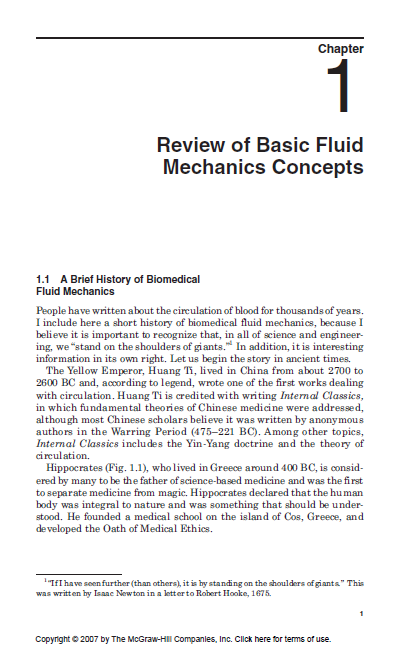
\includegraphics[width=0.45\textwidth]{./chapters/chapter14}
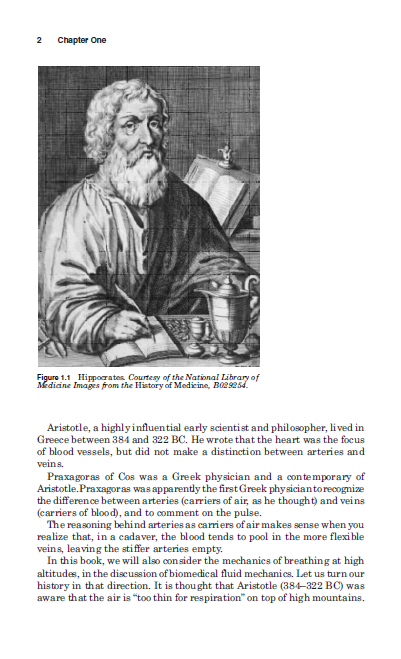
\includegraphics[width=0.45\textwidth]{./chapters/chapter14a}
\end{figure}
\lorem
